\section{Week 1 - Recurrent Neural Networks}
\subsection{Recurrent Neural Networks}
\subsubsection{Why sequence models}
Wide sequence of applications for Sequence models.

\subsubsection{Notation}
Motivation example:
Entity Name recognition, given a sentence X, return y a binary victor with 1 on entities word and 0 otherwise.

\begin{itemize}
    \item $x^{(i)<t>}$ to notate the TIF element in the ith training example.
    \item $T^{(i)}_x$ the length of the ith training example
    \item $y^{(i)<t>}$ tif element in the ith output example
    \item $T^{(i)}_y$ the length of the ith output example
\end{itemize}
To represent a word in a sentence. First define a vocabulary / Dictionary which is a list of the words that you will use in your representations.
Dictionary size in commercial applications can reach 30k, for the largest companies 1M.

One hot representation to repsent the words, e.g. the representation of $x<1>$ (i.e. Harry in the example) is a victor (also known one hot) with 1 at the index of Harry in the dictionnay, 0 everywhere else. You can use work $<UNK>$ for words which are not in your dictionnary.

\subsubsection{Recurrent Neural Network Model}
For mapping X to y, why not a standard network? the problems is that:

\begin{itemize}
    \item Inputs, outputs can be different lengths in different examples.
    \item A naive architecture like this does not share features learned across different positions of text. 
\end{itemize}

Like with CNN we would like things learned for one part of the image to generalize quickly to other parts of the image, and we like a similar effects for sequence data as well.

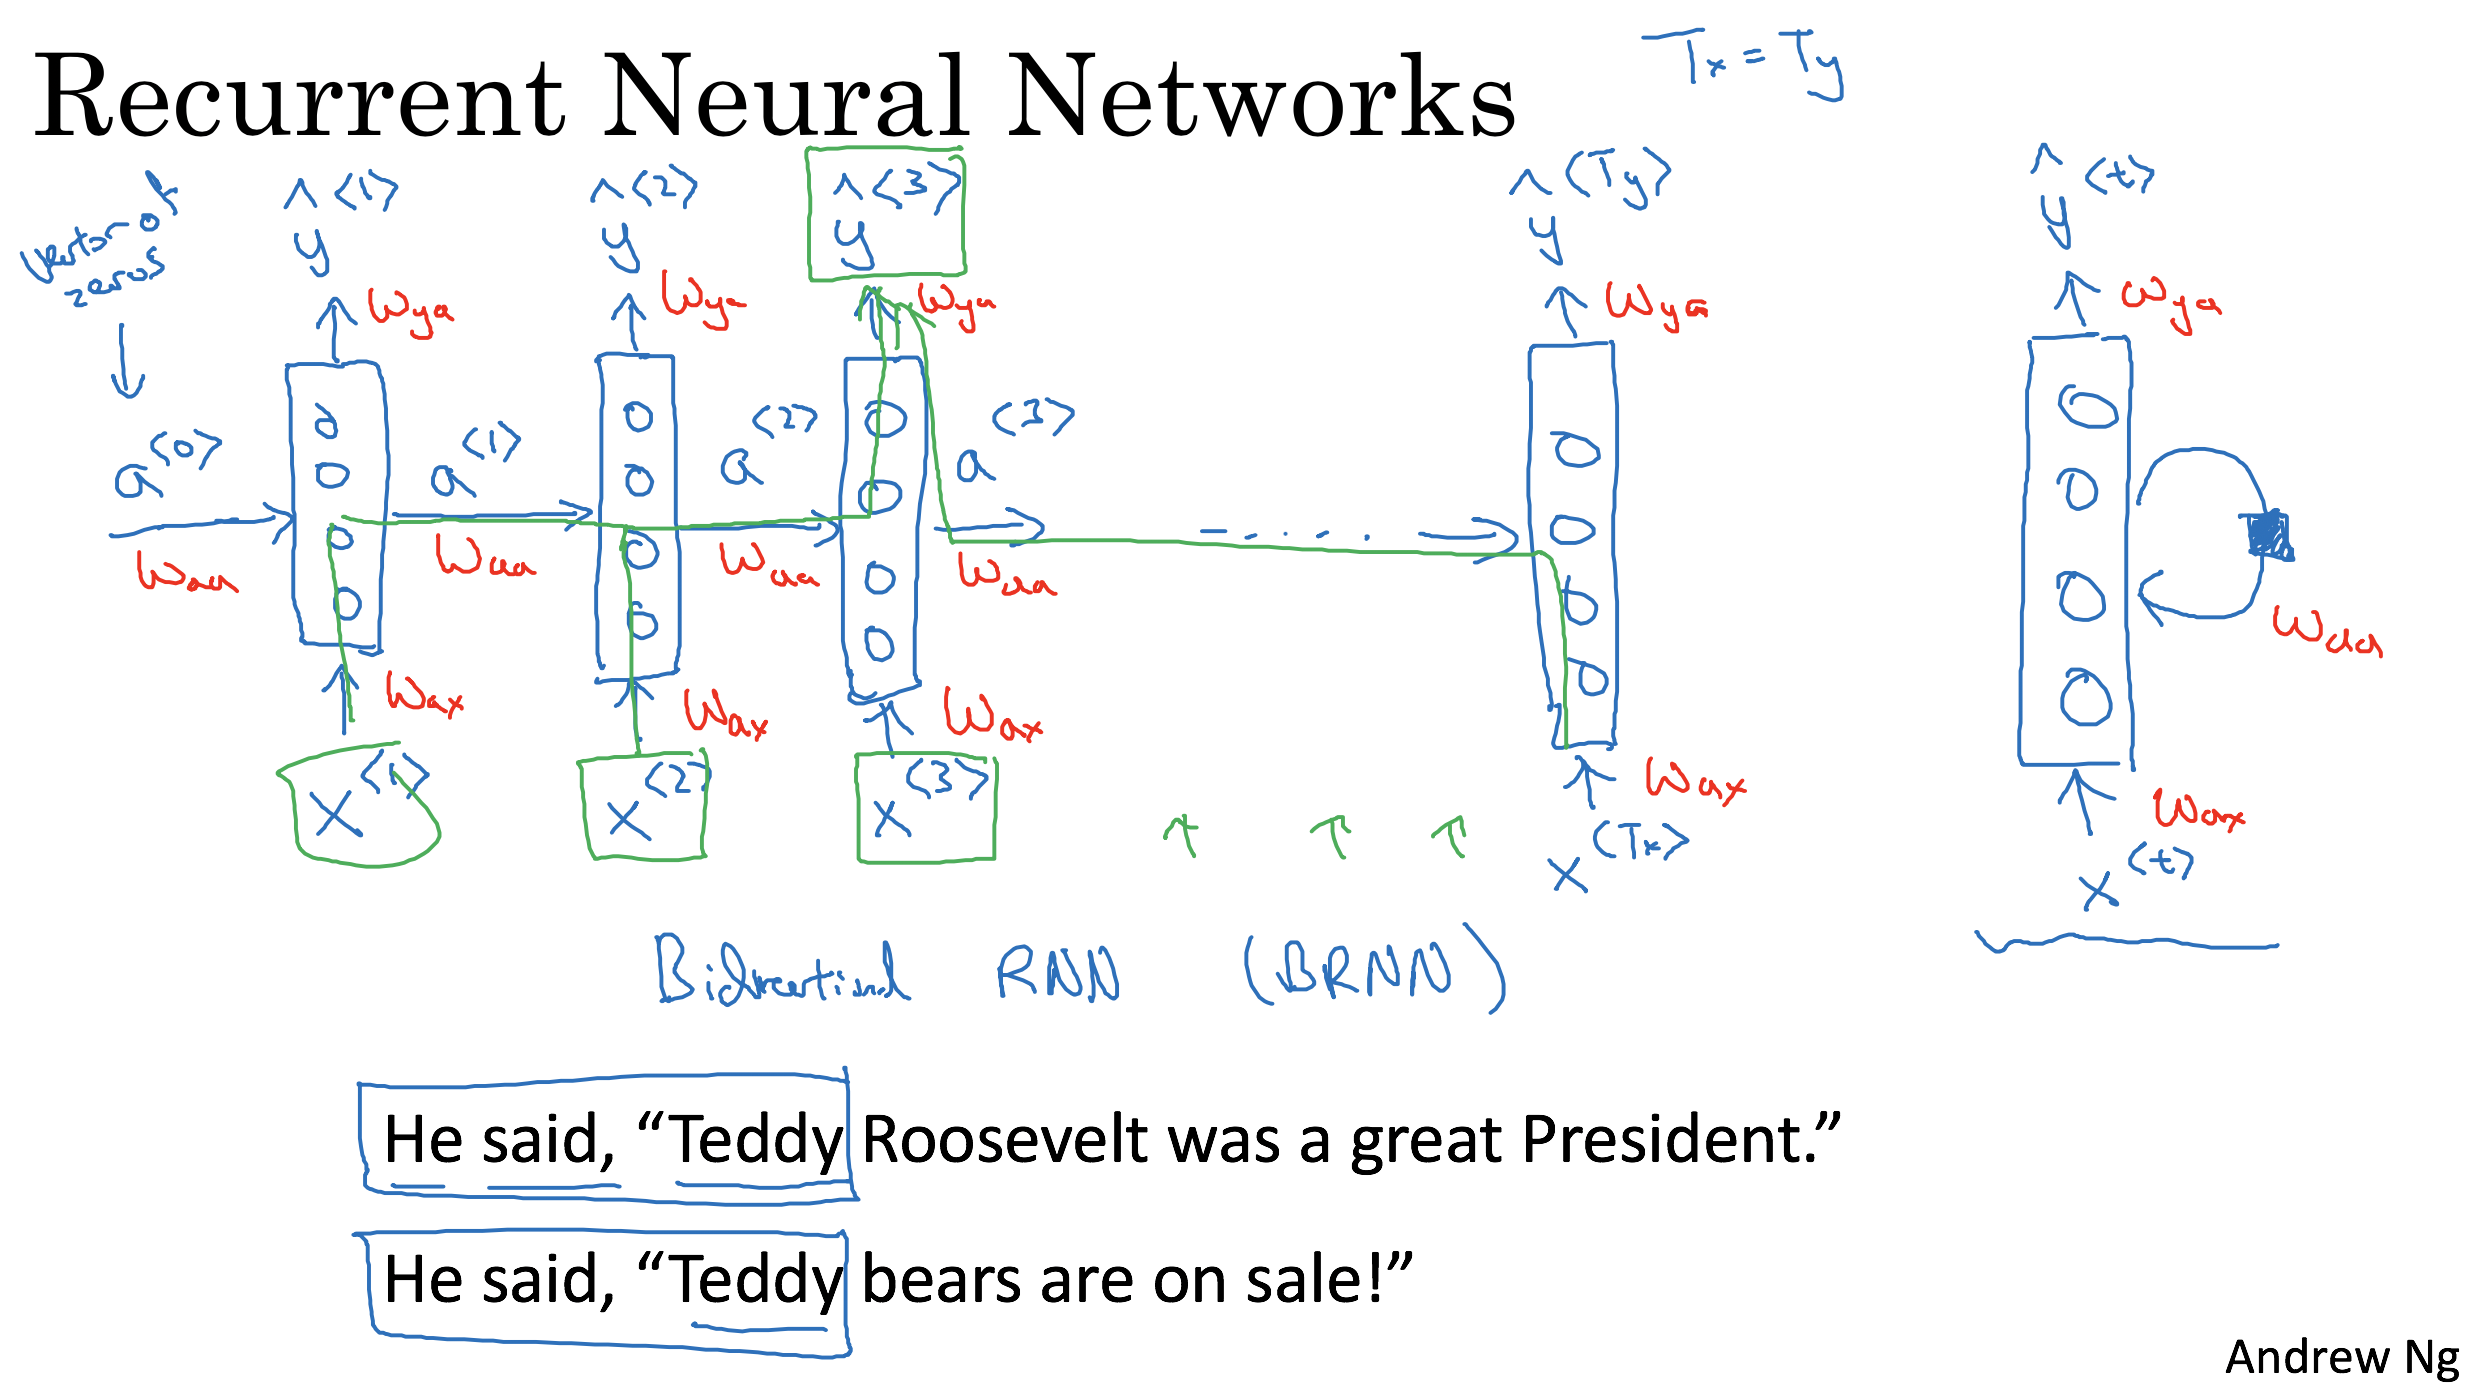
\includegraphics[scale=0.35]{RNN}

If you're reading a sentence from right to left, you pass the first word to the hidden layer, then for the second word you will also passes on the activation of the previous layer. In the first layer, an activation vector of 0s is used. This architecture uses only the previous words, but not the later words, which is a problem. This can be addressed by Bidirectional RNN (BRNN) which we will see later.


The activation function for the hidden units can be tahn or ReLU.
For activation of the output, it can sigmoid if binary, or softmax in case of a k-way classification.

\begin{itemize}
    \item $a^{<0>} = 0$
    \item $a^{<1>} = g(w_{aa} a^{<0>} + w_{ax} x^{<1>} + b_a)$
    \item $\hat{y}^{<1>} = g(w_{ya} a^{<1>} + b_y)$
\end{itemize}

More generaly:
\begin{itemize}
    \item $a^{<t>} = g(w_{aa} a^{<t-1>} + w_{ax} x^{<t>} + b_a)$
    \item $\hat{y}^{<t>} = g(w_{ya} a^{<t>} + b_y)$
\end{itemize}

To simplify the previous general equations, stack the vectors $a^{<t-1>}$, $x^{<t>}$ together, and compress the parameters into one vector parameter:
\begin{itemize}
    \item $a^{<t>} = g(W_{a} [a^{<t-1>}, x^{<t>}])$
    \item $w_{a} = [ w_{aa}, w_{ax} ]$
    \item $\hat{y}^{<t>} = g(w_{y} a^{<t>} + b_y)$
\end{itemize}

\begin{equation*}
    [ w_{aa}, w_{ax} ] \begin{bmatrix}
           a^{<t-1>} \\
           x^{<t>}
         \end{bmatrix} = w_{aa} a^{<t-1>} + w_{ax} x^{<t>}
\end{equation*}

\subsubsection{Backpropagation through time}
It's called through time as you calculate from the right to the left i a decresing time index (back in time), while forward goes from left to right in the increase time.

Standard logistic regression loss, also called the cross entropy loss.
\begin{equation*}
    \mathcal{L}^{<t>} (\hat{y}^{t}, y^{t}) = - y^{t} \log \hat{y}^{t} - (1 - y^{t}) \log(1 - \hat{y}^{t})
\end{equation*}
The loss for the entire sequence:
\begin{equation*}
    \mathcal{L} (\hat{y}, y) = \sum^{T_y}_{t=1} \mathcal{L}^{<t>} (\hat{y}^{t}, y^{t})
\end{equation*}

\subsubsection{Different types of RNNs}
\begin{itemize}
    \item many-to-many: input sequence has many inputs as a sequence and the outputs sequence is also has many outputs. e.g. music generation, starting from note for instance.
    \item many-to-one: it inputs many words and then it just outputs one number, e.g. sentiment classification
    \item one-to-one: a starndard NN, convered in the first course of this sequence
\end{itemize}

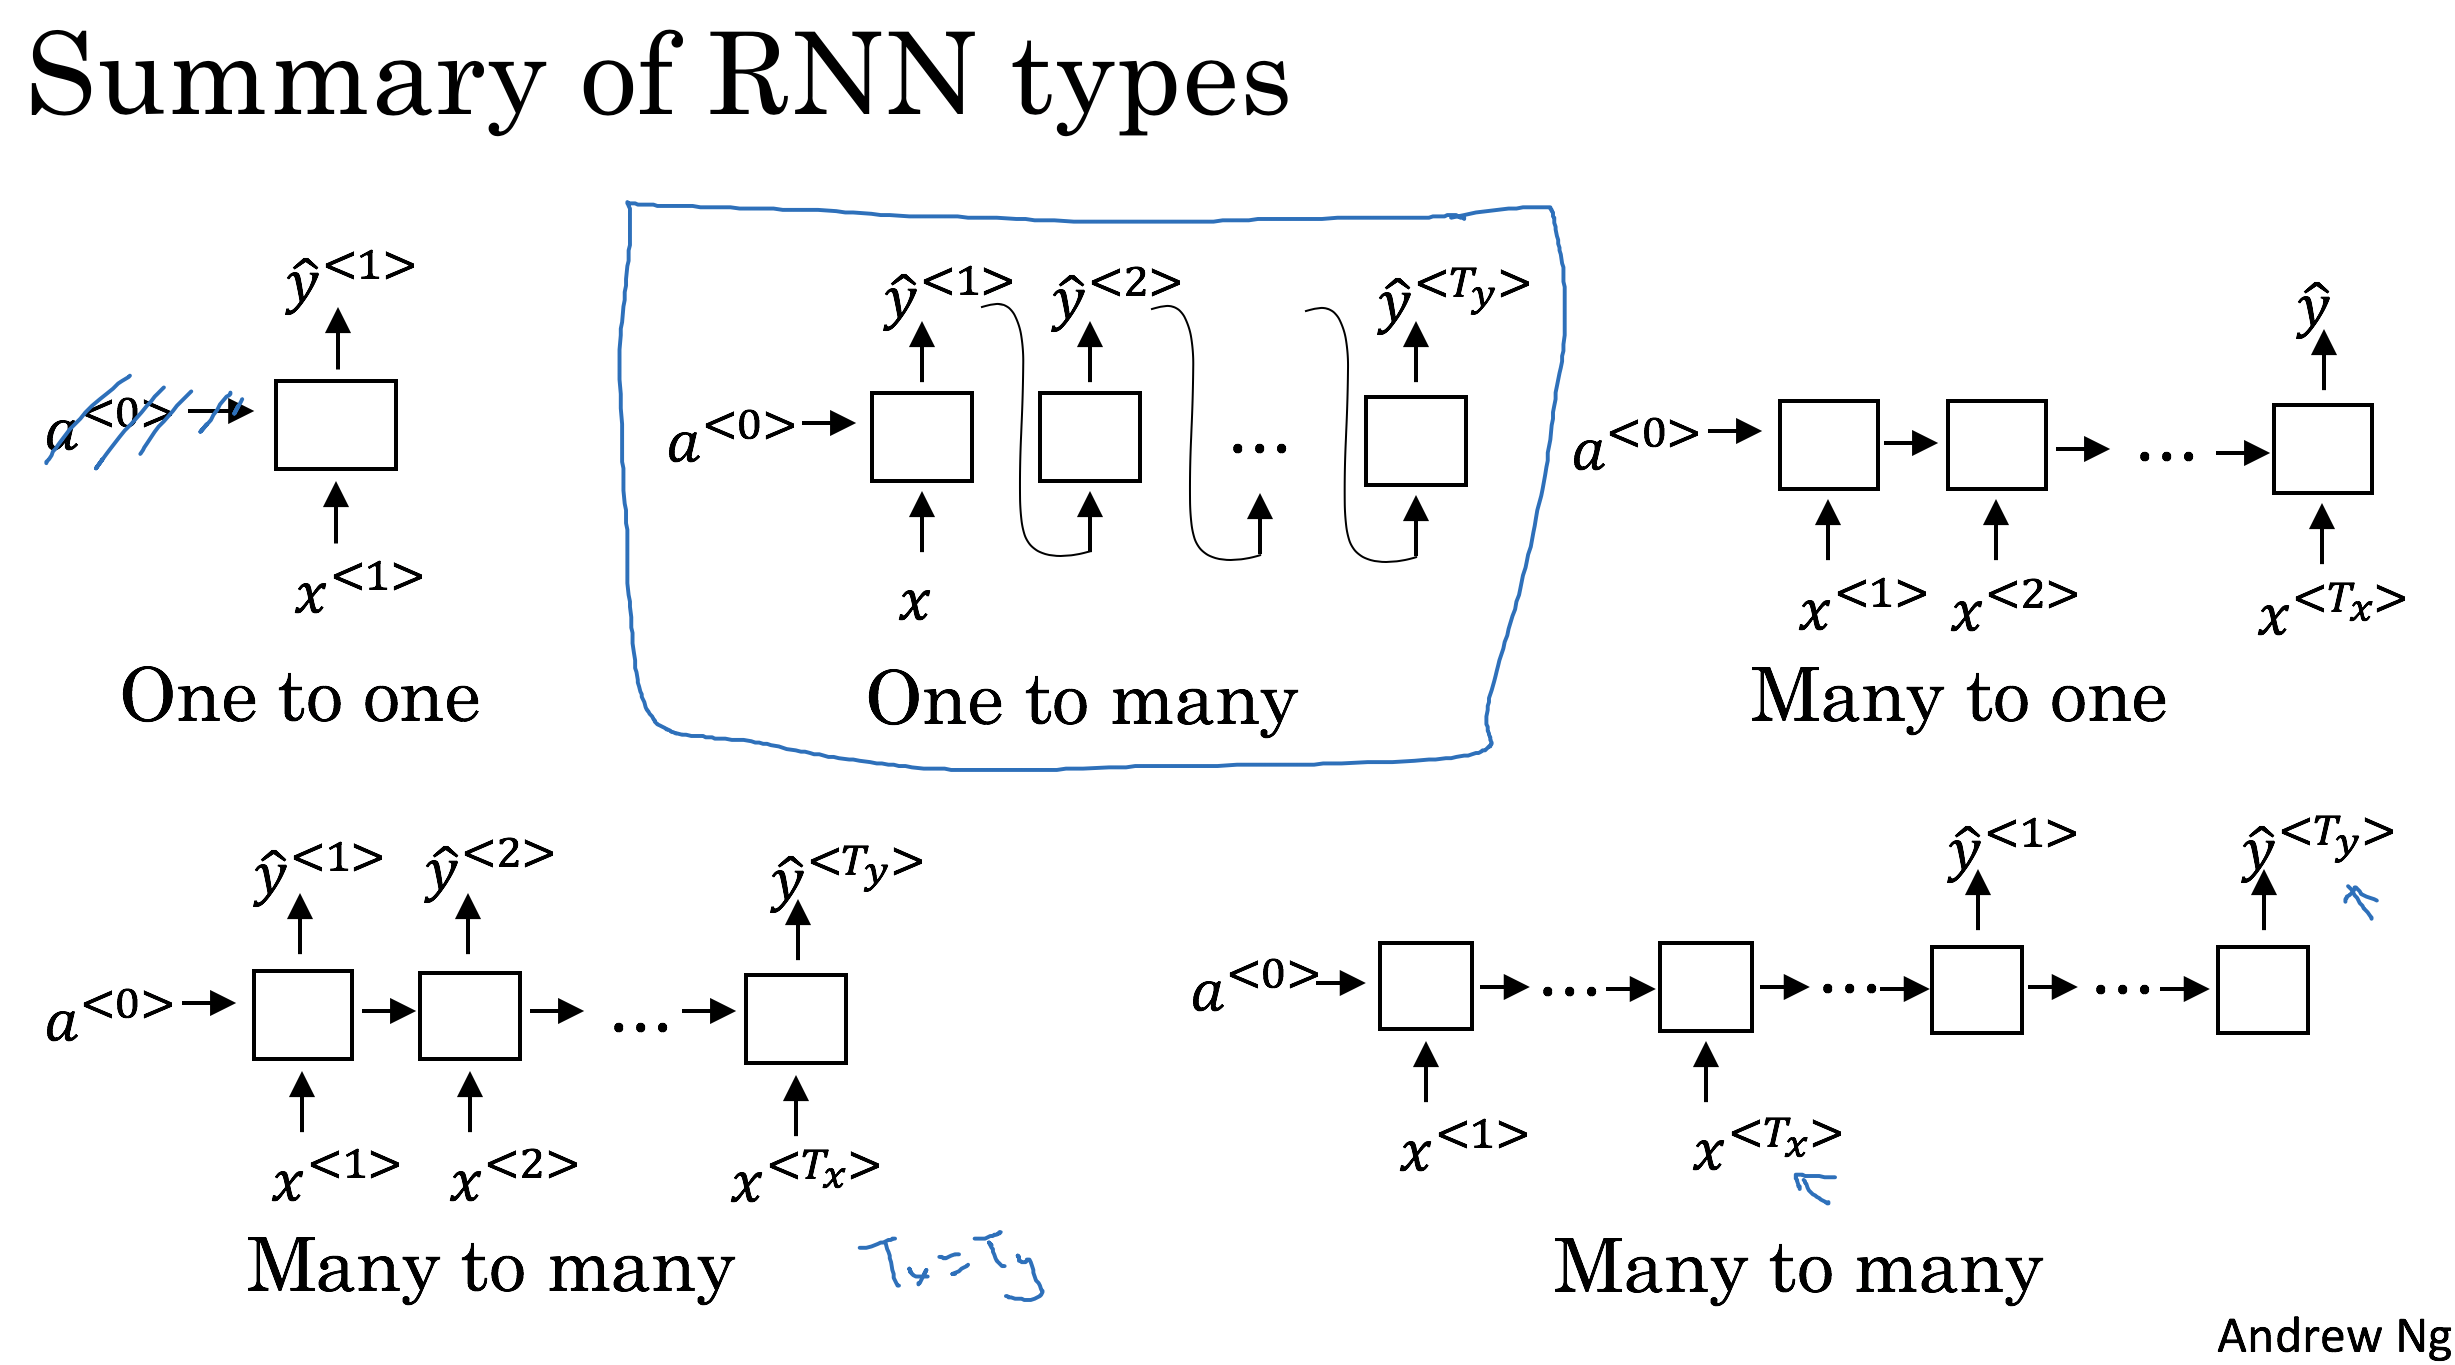
\includegraphics[scale=0.35]{RNN_Architectures}

\subsubsection{Language model and sequence generation}
Language model, choose between two sentences based on a probability to decide which one is more likely. A language modeal, given any sentence, does tell you what is the probability of that particular sentence.

Build a language model with an RNN, training set: large corpus of english text. For the model to capture the end of sentence, add to each training sentence the $<EOS>$ token at its end.

 RNN model:
 What that's going to be $y^{<1>}$: this step has a soft max it's trying to predict. What is the probability of any word in the dictionary? it would be a 10,000 way soft max output, or 10,002, if we call unknown word and end of the sentence is two additional tokens.
 
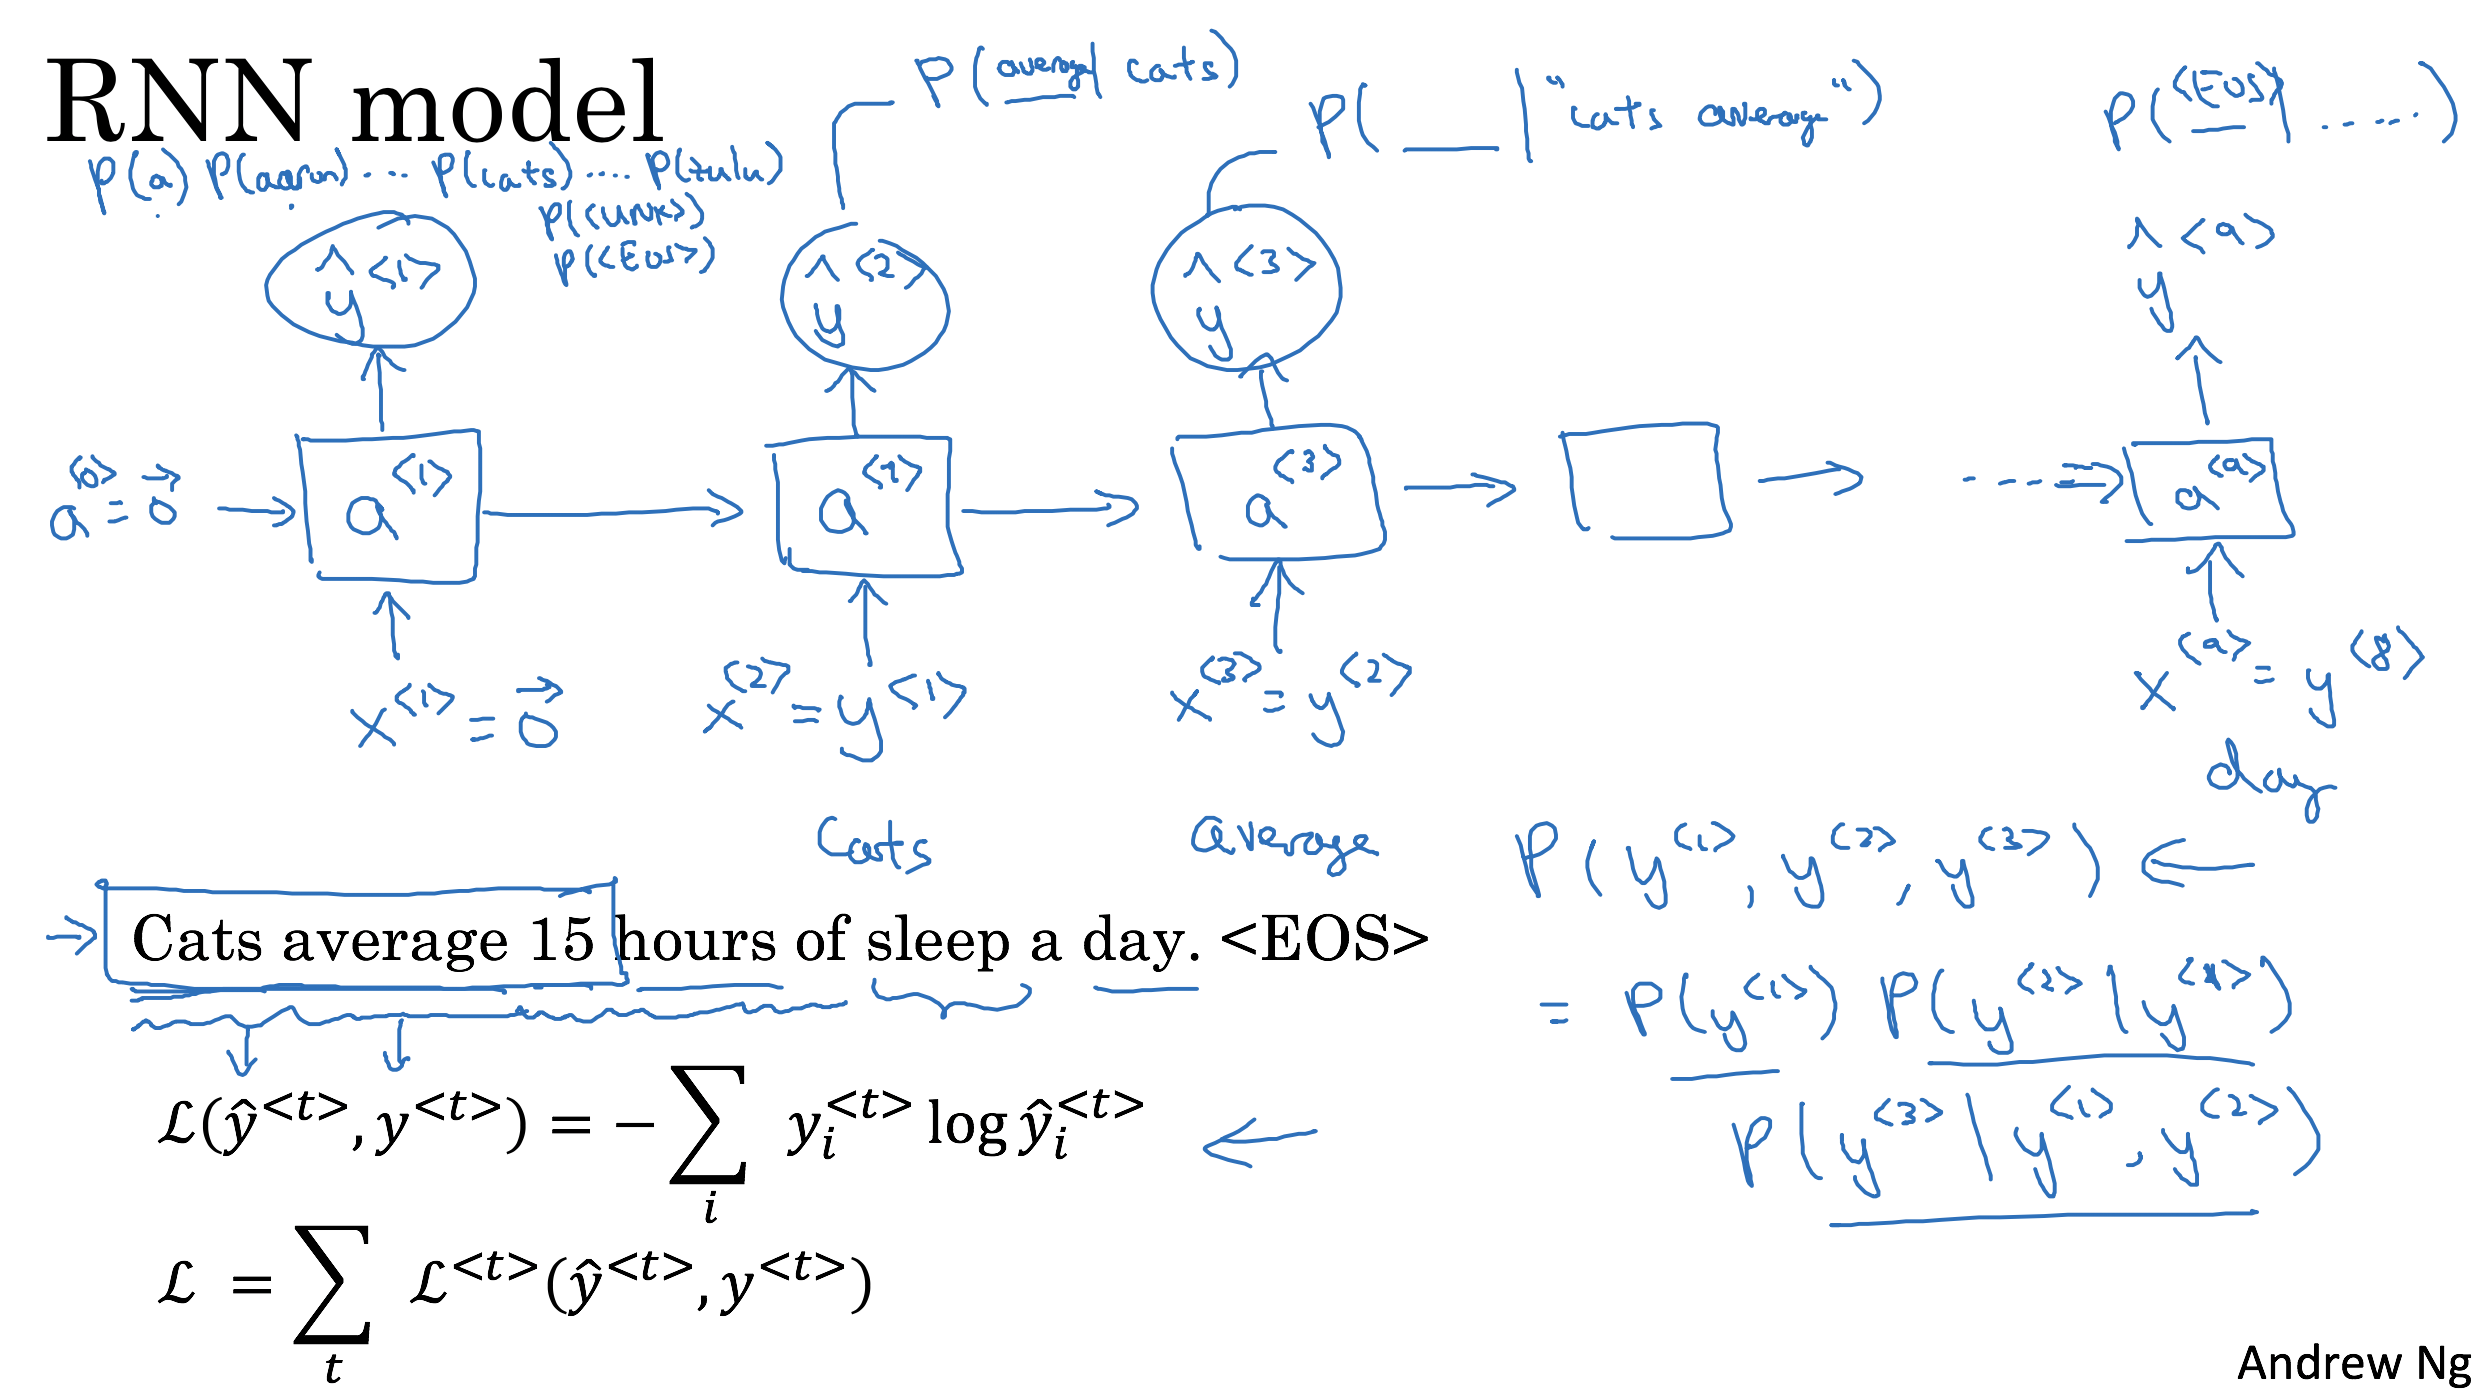
\includegraphics[scale=0.35]{RNN_model}
 The output of the previous layer in passed to the next one, ie $x^{<t>}=y^{<t>}$, this RNN learns to generate a word a time by looking at all the previous ones.
 
 Given a three words sentence, $y^{<1>}$, $y^{<2>}$, $y^{<3>}$. Predict the probability to see this words in sequence:
\begin{equation}
 P (y^{<1>}, y^{<2>}, y^{<3>}) = P(y^{<1>}) P(y^{<2>} | y^{<1>}) P(y^{<3>} | y^{<1>}, y^{<2>})
\end{equation}
It turns out one of the most fun things you could do with a language model is to sample sequences from the model. 


\subsubsection{Sampling novel sequences}
After training a \textbf{sequence model}, one of the ways to informally get a sense of what is learned is to have a sample novel sequences.

After training a sequence model, input an X=0, then from the output $y^{<1>}$ which is 10k way softmax, then sample one word of this distribution and pass it to the next step/timestamp, etc, until you get to the end. To detect the end of sentence, wait until you see $<EOS>$ in the output. This is how to generate a randomly sampled sentence.

\begin{figure}[H]
\centering
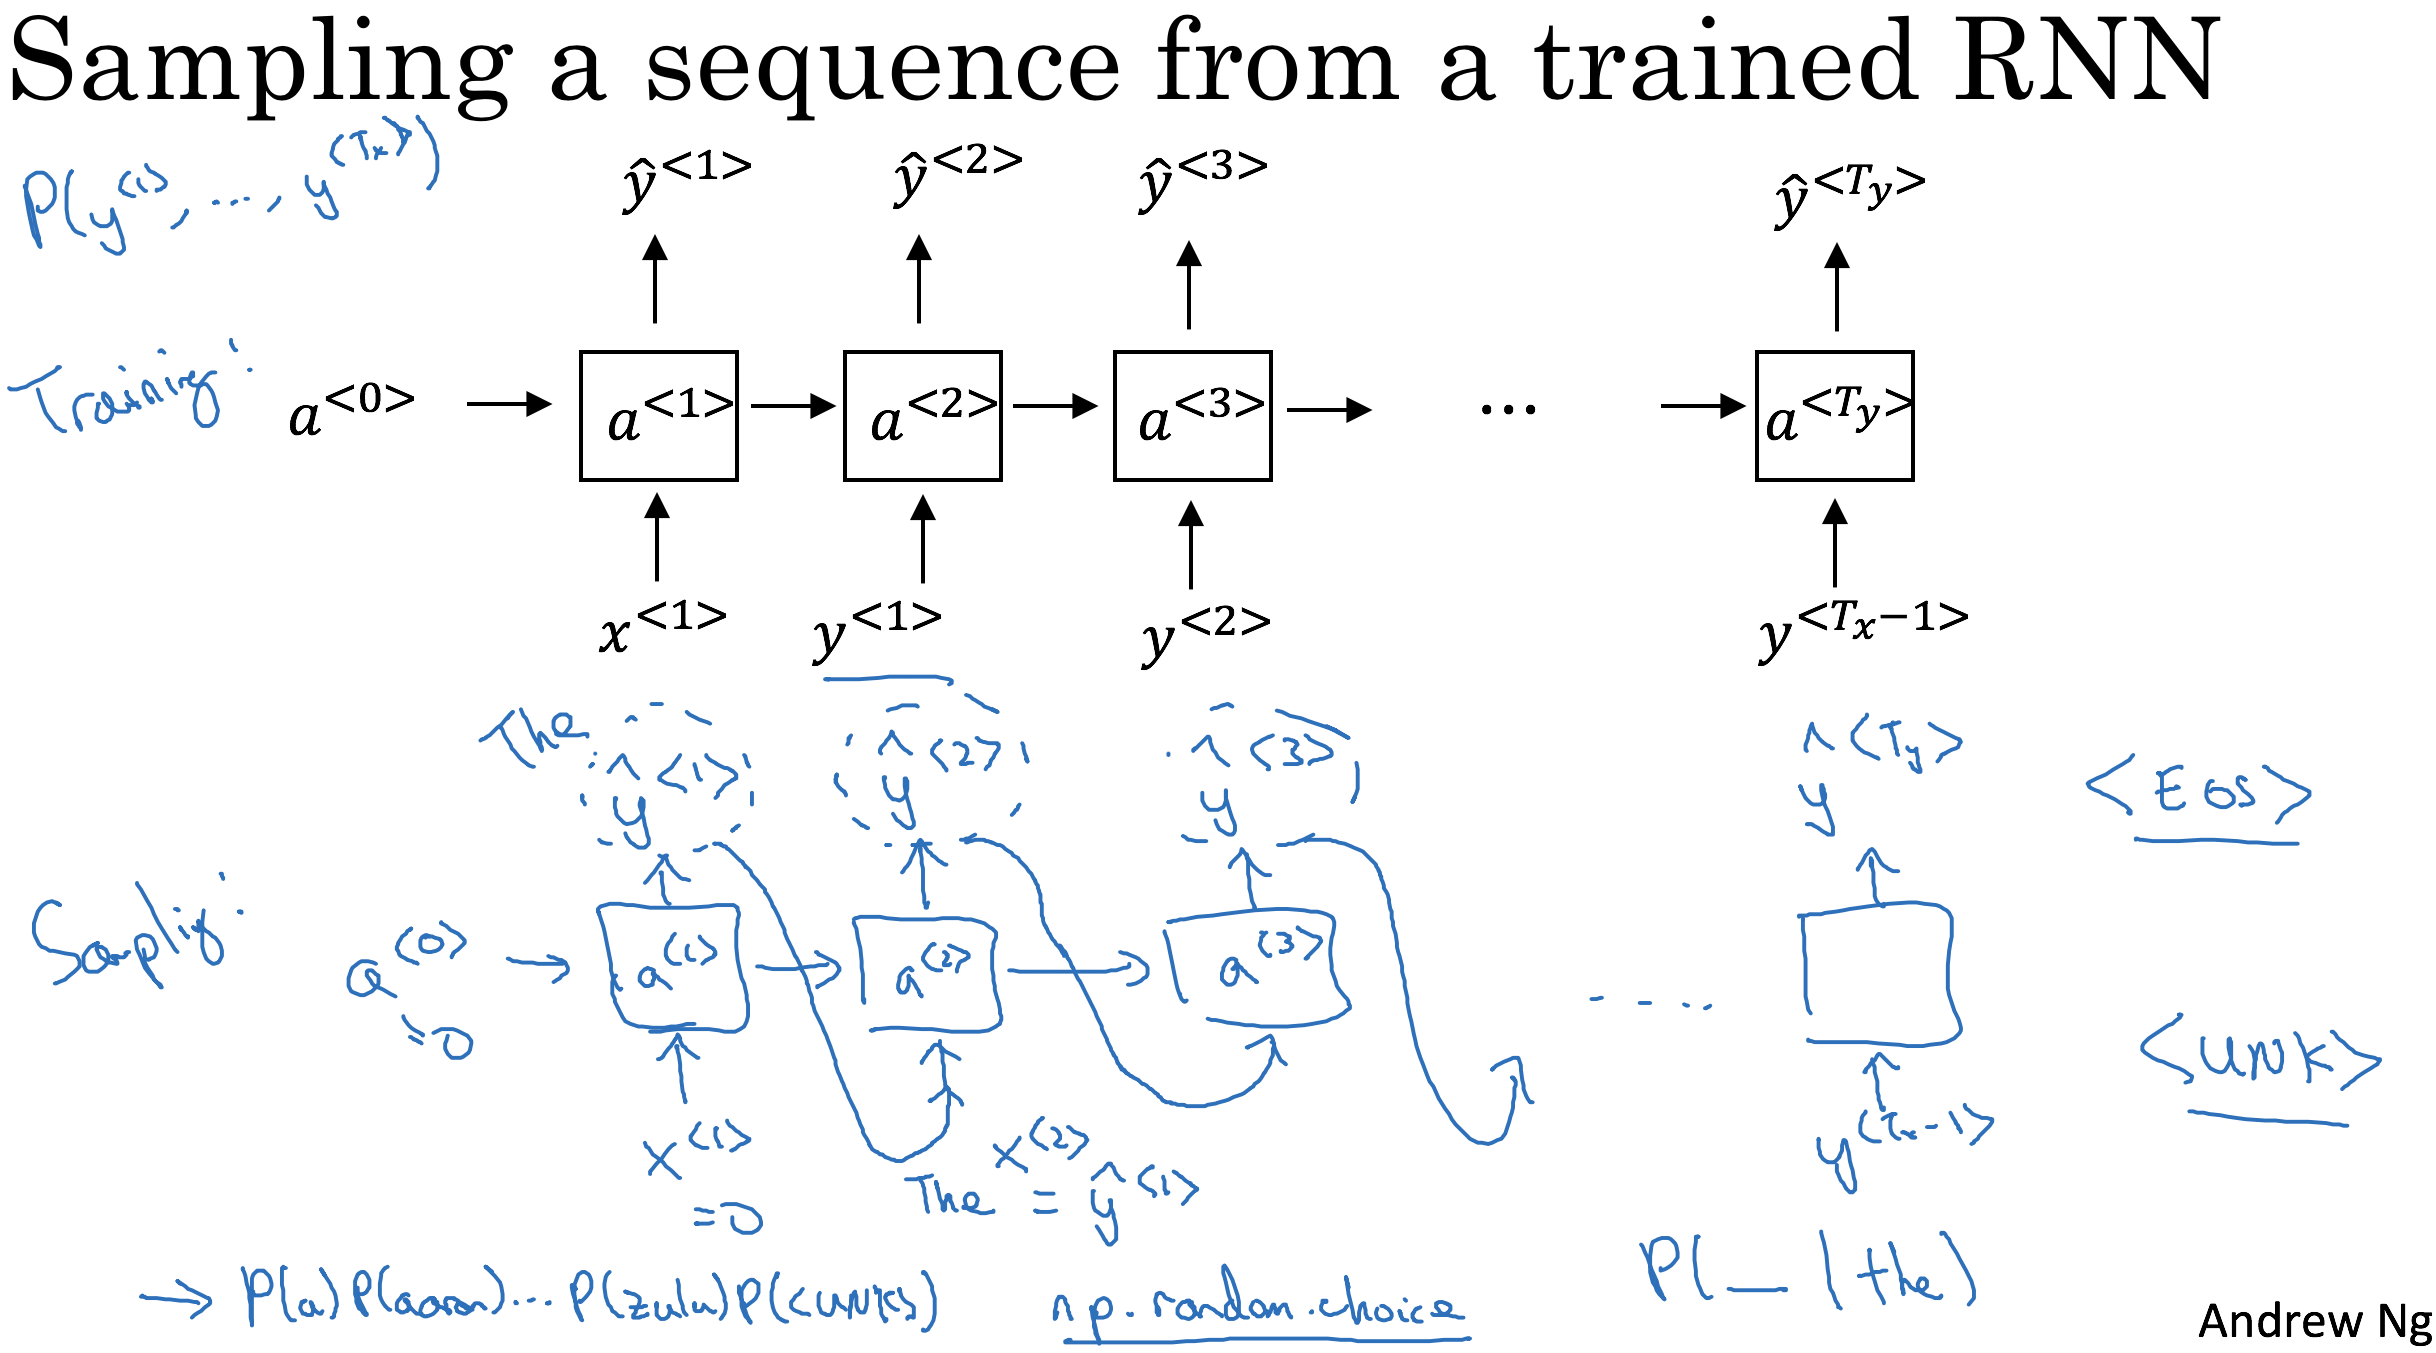
\includegraphics[scale=0.35]{RNN_Sampling_Sentence}
\caption{Sampling a sequence from a trained RNN}
\end{figure}

Character-level language mode:
In this case, the vocabulary is a sequence of alphabet characters, e.g. Vocabulary = [a, b, c, ..., z, space, dot, comma, 0, ..., 9, A, ..., Z].

The main disadvantage of the character level language model is that:
\begin{itemize}
    \item you end up with much longer sequences. So many english sentences will have 10 to 20 words but may have many, many dozens of characters.
    \item And so character language models are not as good as word level language models at capturing long range dependencies between how the the earlier parts of the sentence also affect the later part of the sentence. 
    \item And character level models are also just more computationally expensive to train.
\end{itemize}

\subsubsection{Vanishing gradients with RNNs}
One of the problemns of basic RNN is that it runs into vanishing gradients and exploding problems:
An example of long term dependencies in a laguage: when outputing 'cat' later we should have 'was', similarly when outputting 'cats' we should have 'were'. 
In a deep NN, gradient have hard time propagating back, i.e. errors associated with later timestamps have hard time impacting erros in earlier timestamps.
RNN output is influced by locality, i.e, timestamps nearby. For this, RRN are not good at capturing \textbf{Long range dependencies}.

Similarly, if gradient becomes too big \textbf{Expliding gradients} (i.e. NaN) as function of number of layers, then apply gradient clipping. i.e. look at your gradient vectors, and if it is bigger than some threshold, re-scale some of the gradient vector so that is not too big. So there are clips according to some maximum value.


\subsubsection{Gated Recurrent Unit (GRU)}
It's a modification to the RNN hidden layer that makes it much better capturing long range connections and helps a lot with the vanishing gradient problems.

\begin{figure}[H]
\hfill
\subfigure[Gradient Recurrent Unit]{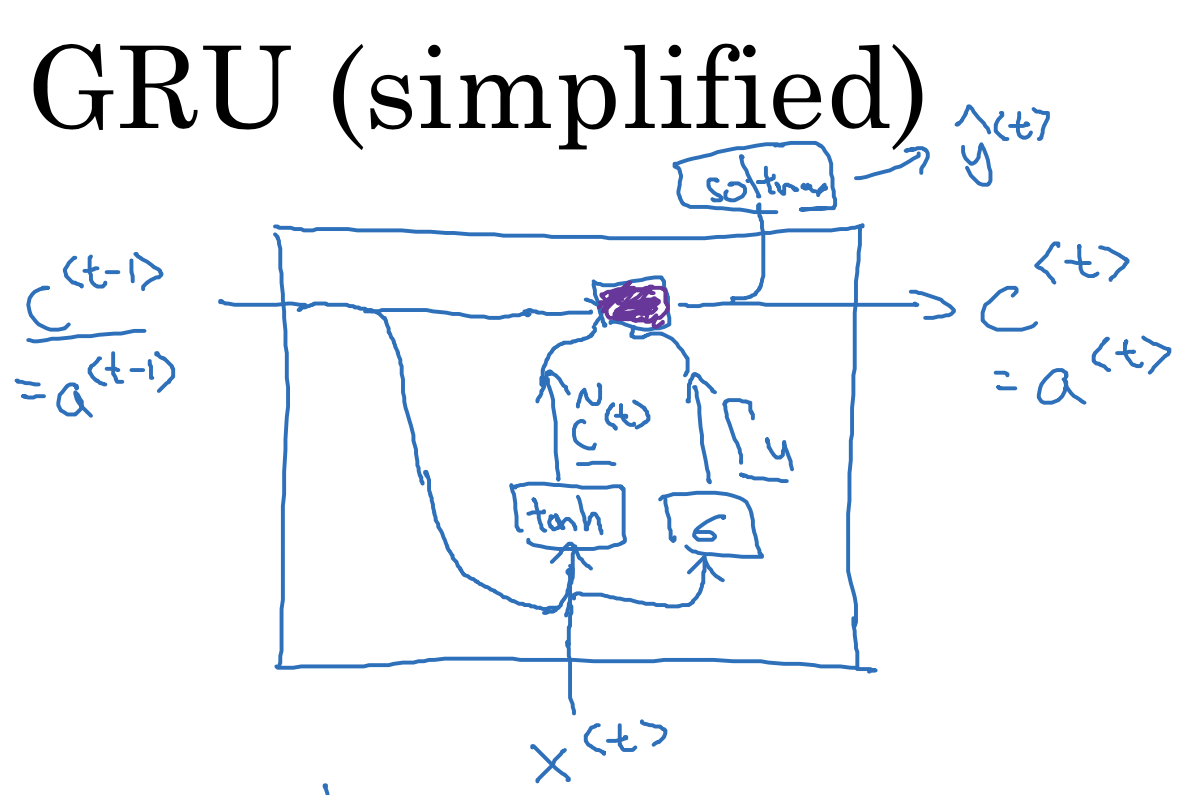
\includegraphics[scale=0.4]{RNN_GRU}}
\hfill
\subfigure[Recurrent basic unit]{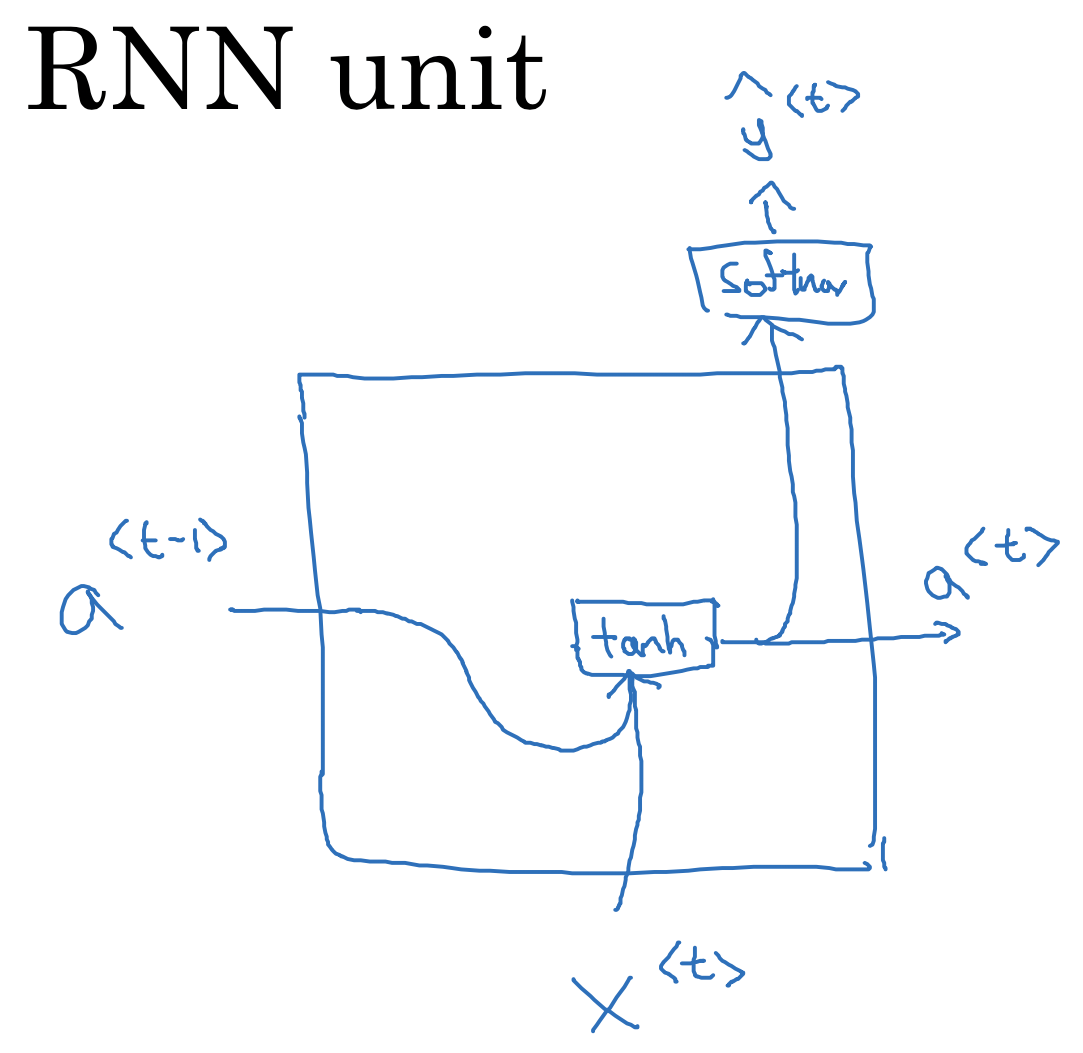
\includegraphics[scale=0.35]{RNN_basic}}
\hfill
\caption{RNN units}
\end{figure}

Memory cell at t, $C^{<t>} = a^{<t>}$ then $\hat{C}^{<t>} = \text{tanh}(w_c[C^{<t-1>}, x^{<t>}] + b_c)$
The important idea is to have a \textbf{gate}, alway zero or one, in practice it's calculated using a sigmoid function, which has a role to decide when to use a word. With 'u' stands for update, the formula is:
\begin{equation*}
  \Gamma_u = \sigma (w_u[C^{<t-1>}, x^{<t>}] + b_u)
\end{equation*}

\begin{equation*}
C^{<t>} = \Gamma_u * \hat{C}^{<t>} + (1 - \Gamma_u) * C^{<t-1>}
\end{equation*}

\texttt{Full GRU}
Many different possible versions of how to design these units, to try to have longer range connections, to try to have more the longer range effects and also address vanishing gradient problems. And the GRU is one of the most commonly used versions. e.g, full GRU formula is:




\begin{figure}[!ht]
  \begin{equation}
    \hat{C}^{<t>} = \text{tanh}(w_c[\Gamma_r * C^{<t-1>}, x^{<t>}] + b_c)
  \end{equation}
\caption{The candidate for replacing the memory cell}
\end{figure}

\begin{equation*}
  \Gamma_u = \sigma (w_u[C^{<t-1>}, x^{<t>}] + b_u)
\end{equation*}
\begin{equation*}
  \Gamma_r = \sigma (w_r[C^{<t-1>}, x^{<t>}] + b_r)
\end{equation*}
Use the gate $\Gamma_u$ to decide whether or not to update the memory cell.
\begin{equation*}
C^{<t>} = \Gamma_u * \hat{C}^{<t>} + (1 - \Gamma_u) * C^{<t-1>}
\end{equation*}

\subsubsection{Long Short Term Memory (LSTM)}
A more powerful and general GRU version. It has three gates instead of two an place them in different places:
\begin{itemize}
    \item $\Gamma_u$ the update gate
    \item $\Gamma_f$ the forget gate
    \item $\Gamma_o$ the output gate
\end{itemize}

\begin{figure}[H]
\centering
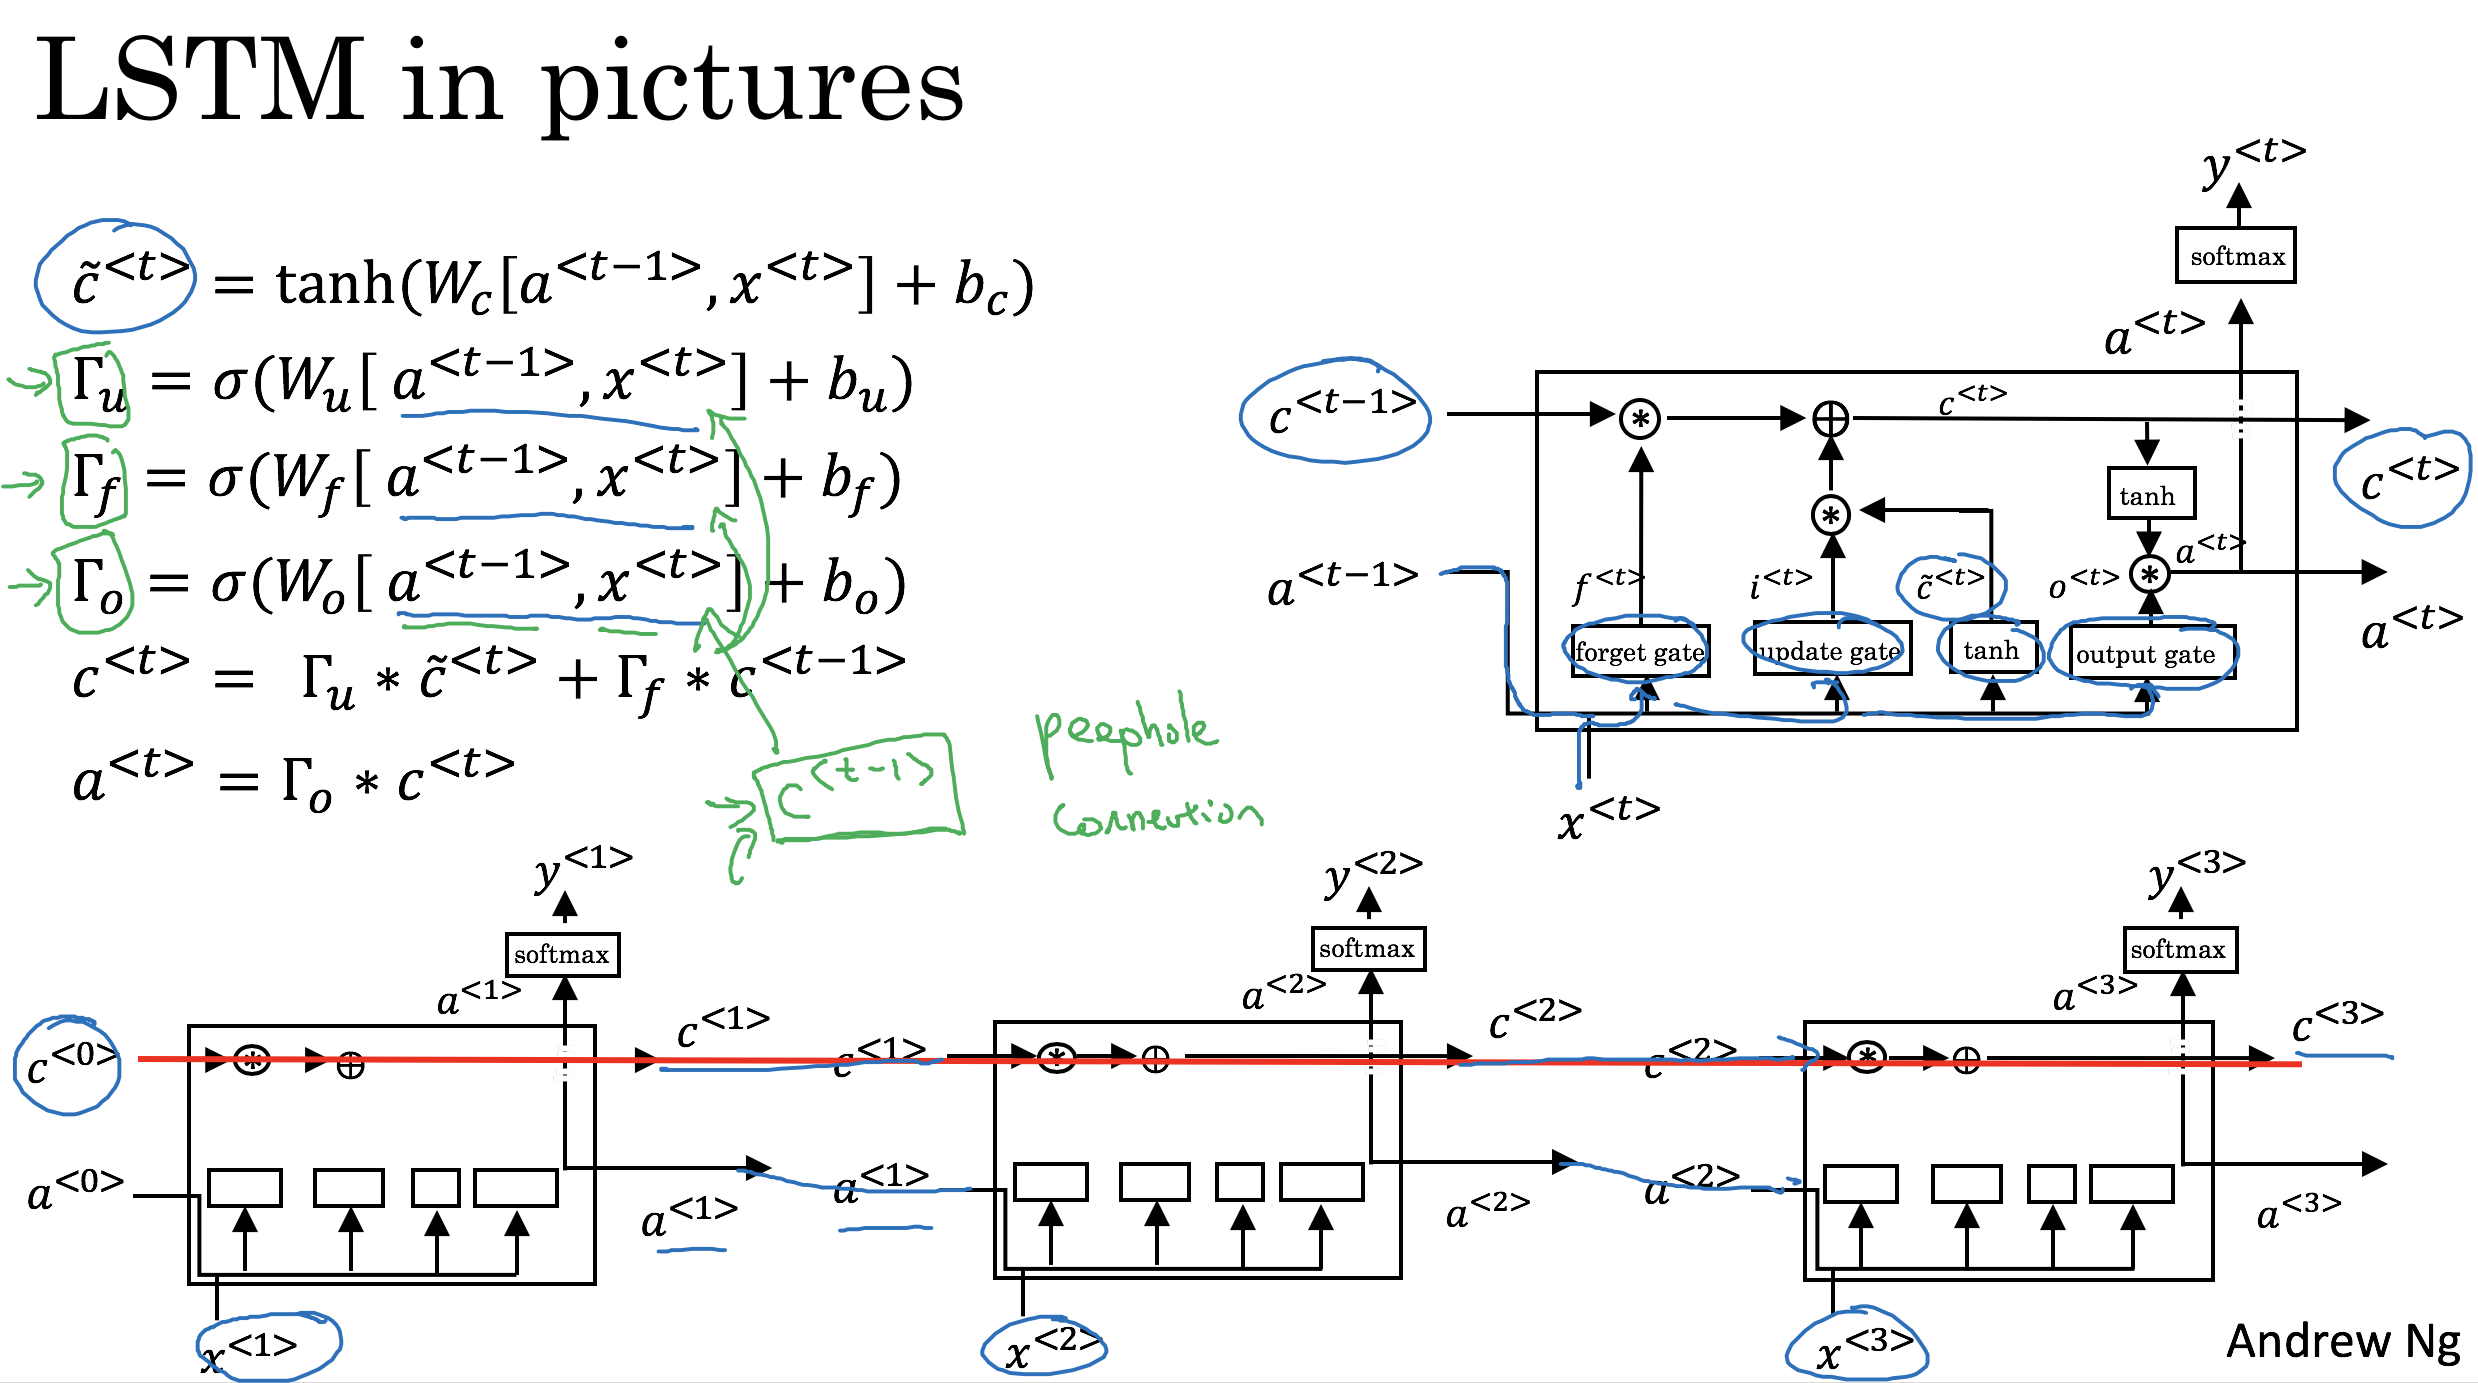
\includegraphics[scale=0.35]{RNN_LSTM}
\caption{LSTM}
\end{figure}
\textbf{Peephole connection} mean that $c_t$ minus one is used to affect the gate value as well.

\begin{itemize}
    \item The advantage of the GRU is that it's a simpler model and so it is actually easier to build a much bigger network, it only has two gates, so computationally, it runs a bit faster. So, it scales the building somewhat bigger models. 
    \item the LSTM is more powerful and more effective since it has three gates instead of two. If you want to pick one to use, I think LSTM has been the historically more proven choice. 
\end{itemize}

\begin{figure}[H]
\centering
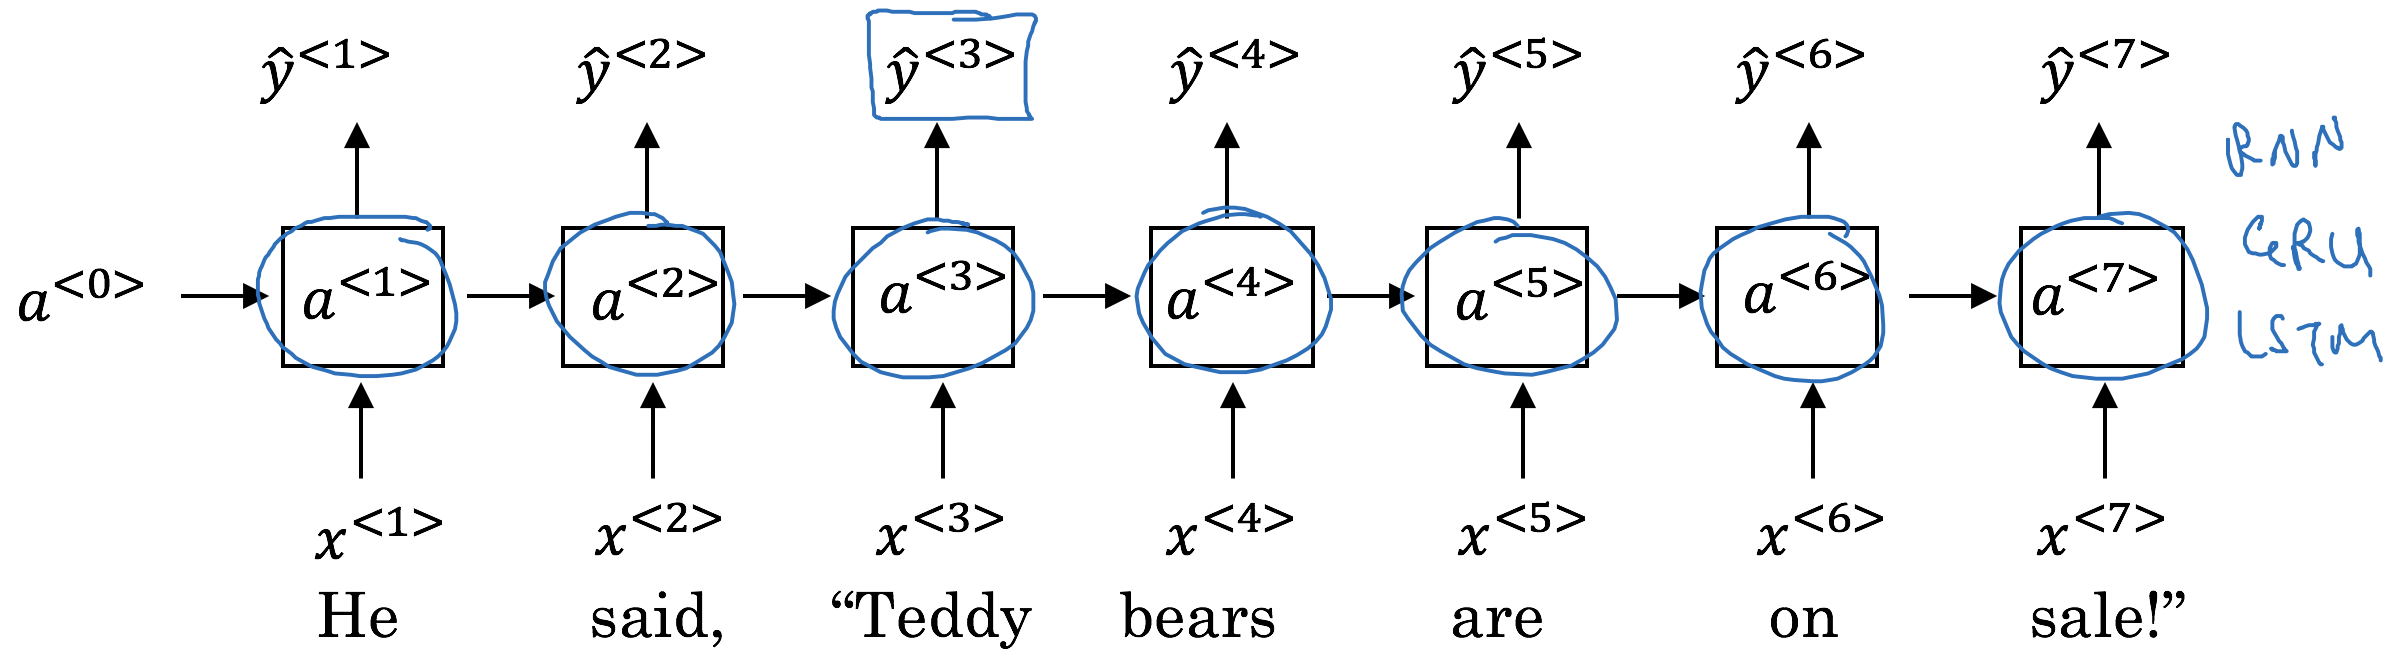
\includegraphics[scale=0.35]{RNN_example_blocks_net}
\caption{Example of network of RNN,GRU,LSTM blocks}
\end{figure}

\subsubsection{Bidirectional RNN}In a BRNNinformation from $x^{[1]}$ can flow forward to $\hat{y}^{<3>}$ through $\vec{a}^{<1>}$, $\vec{a}^{<2>}$ and  $\vec{a}^{<3>}$. Information can also flow backward from $x^{[4]}$ to $\overleftarrow{a}^{[4]}$ to backward $\overleftarrow{a}^{[y]}$ and finally $\hat{y}^{<3>}$.

This allows the prediction of output to take information from the past as well as from the future.
\begin{figure}[H]
\centering
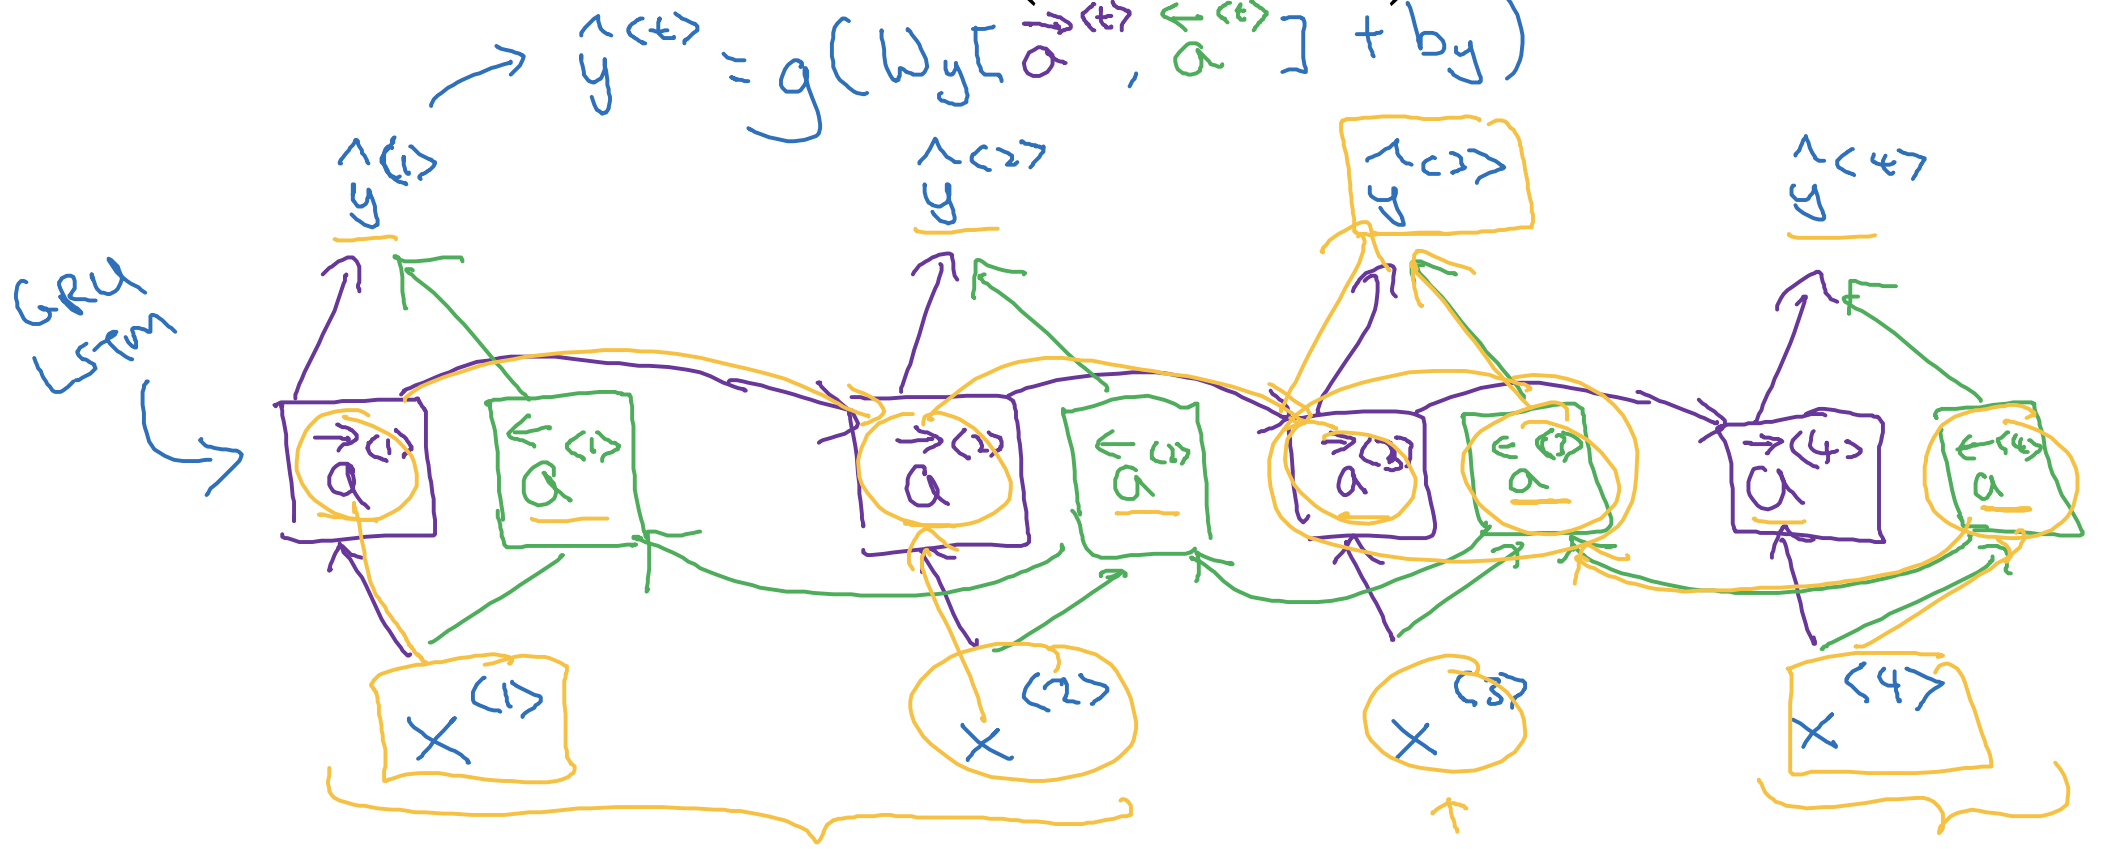
\includegraphics[scale=0.35]{RNN_bidirectional}
\caption{Example acyclic graph for BRNN}
\end{figure}
In this figure, the blocks can be basic RNN blocks, GRU or LSTM.

The disadvantage is that you need the entire sequence before you actually start processing, e.g. in speech recognition, you need the person to stop talking to start processing.

\subsubsection{Deep RNNs}
To learn complex functions, it is useful to stack many layers of RNN.
\begin{figure}[H]
\centering
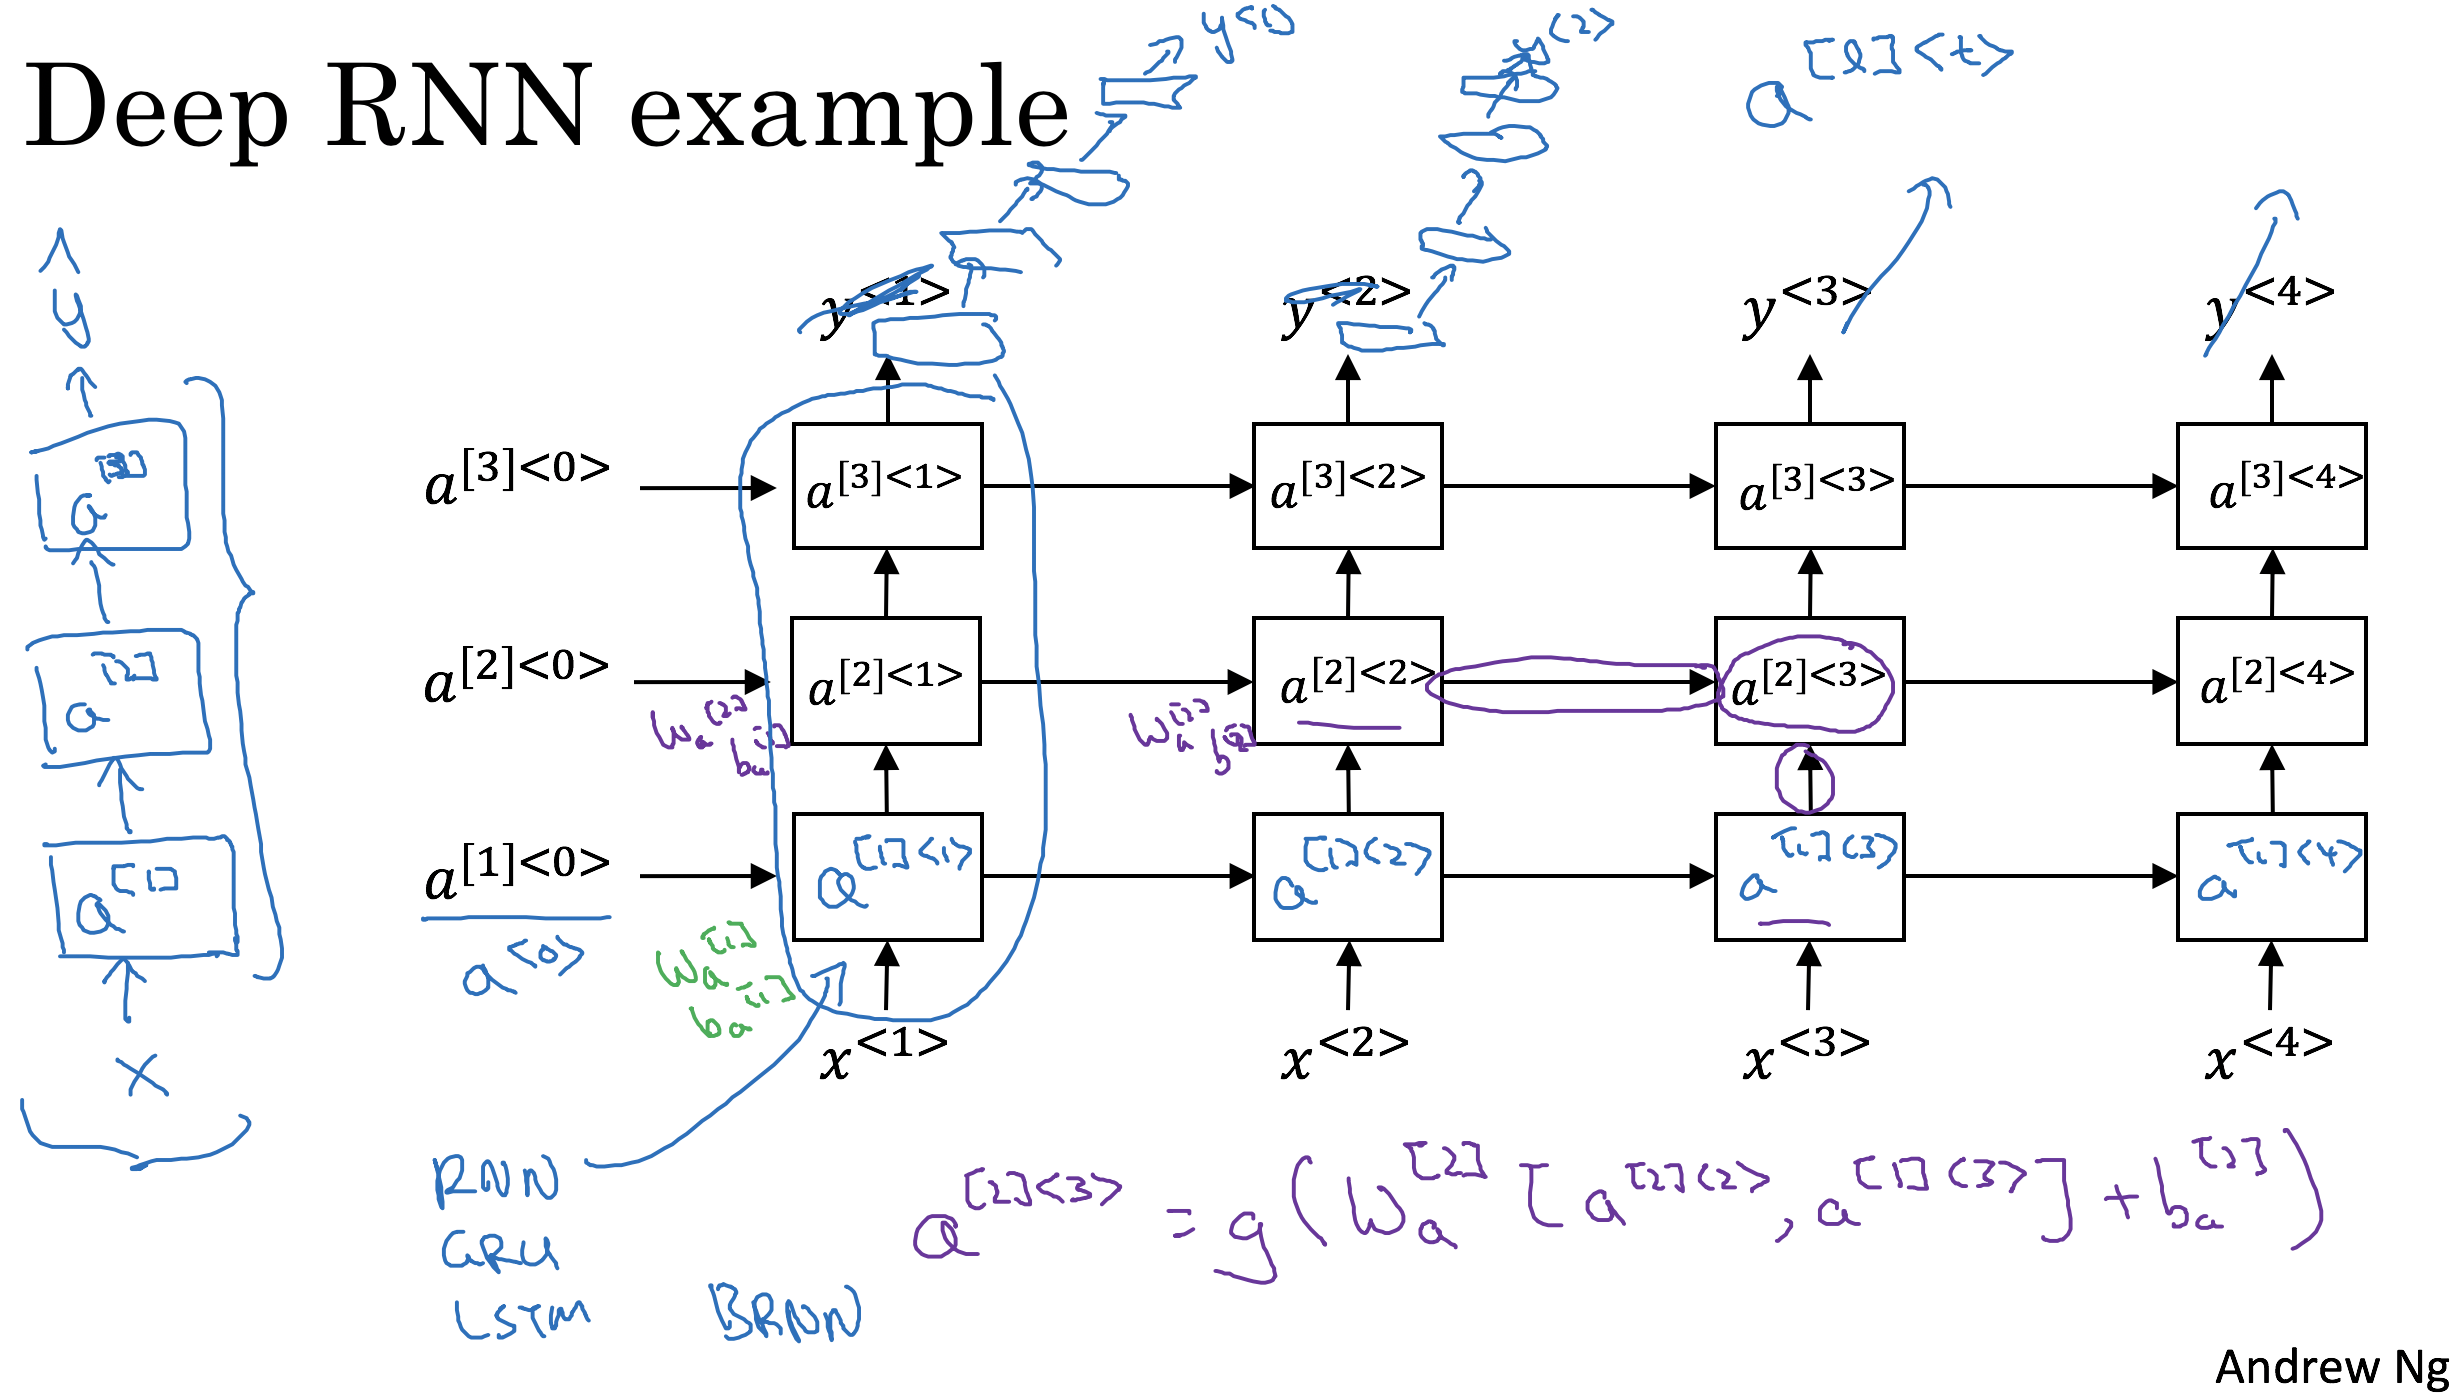
\includegraphics[scale=0.35]{RNN_Deep}
\caption{Example of DeepRNN with 3 layers}
\end{figure}
Example of how to calculate activation function:
\begin{equation*}
    a^{{[2]}<3>} = g(w^{[2]}_a [ a^{{[2]}<2>}, a^{{[1]}<3>} ] + b^{<3>}_a )
\end{equation*}

\subsection{Practice questions}


\subsubsection{QUIZ - Recurrent Neural Networks}
\textbf{1.} Suppose your training examples are sentences (sequences of words). Which of the following refers to the $j^{th}$  word in the $i^{th}$ training example?
\begin{itemize}
    \item $x^{(i)<j>}$ (XConsider this RNN:)
    \item $x^{<i>(j)}$
    \item $x^{(j)<i>}$
    \item $x^{<j>(i)}$
\end{itemize}
\textbf{2.} Consider this RNN:
This specific type of architecture is appropriate when:
\begin{itemize}
    \item $T_x = T_y$ (X)
    \item $T_x < T_y$
    \item $T_x > T_y$
    \item $T_x = 1$
\end{itemize}
\textbf{3.} To which of these tasks would you apply a many-to-one RNN architecture? (Check all that apply).
\begin{itemize}
    \item Speech recognition (input an audio clip and output a transcript)
    \item Sentiment classification (input a piece of text and output a 0/1 to denote positive or negative sentiment) (X)
    \item Image classification (input an image and output a label)
    \item Gender recognition from speech (input an audio clip and output a label indicating the speaker’s gender) (X)
\end{itemize}
\textbf{4.} You are training this RNN language model.
At the $t^{th}$ time step, what is the RNN doing? Choose the best answer.
\begin{itemize}
    \item Estimating $P(y^{<1>}, y^{<2>}, ..., y^{<t-1>})$
    \item Estimating $P(y^{<t>})$
    \item Estimating $P(y^{<t>} \mid y^{<1>}, y^{<2>}, ..., y^{<t-1>})$ (X)
    \item Estimating $P(y^{<t>} \mid y^{<1>}, y^{<2>}, ..., y^{<t>})$
\end{itemize}
\textbf{5.} You have finished training a language model RNN and are using it to sample random sentences, as follows:
What are you doing at each time step $t$?
\begin{itemize}
    \item (i) Use the probabilities output by the RNN to pick the highest probability word for that time-step as $\hat{y}^{<t>}$. (ii) Then pass the ground-truth word from the training set to the next time-step.
    \item (i) Use the probabilities output by the RNN to randomly sample a chosen word for that time-step as $\hat{y}^{<t>}$. (ii) Then pass the ground-truth word from the training set to the next time-step.
    \item (i) Use the probabilities output by the RNN to pick the highest probability word for that time-step as $\hat{y}^{<t>}$. (ii) Then pass this selected word to the next time-step.
    \item (i) Use the probabilities output by the RNN to randomly sample a chosen word for that time-step as $\hat{y}^{<t>}$. (ii) Then pass this selected word to the next time-step. (X)
\end{itemize}
\textbf{6.} You are training an RNN, and find that your weights and activations are all taking on the value of NaN (“Not a Number”). Which of these is the most likely cause of this problem?
\begin{itemize}
    \item Vanishing gradient problem.
    \item Exploding gradient problem. (X)
    \item ReLU activation function g(.) used to compute g(z), where z is too large.
    \item Sigmoid activation function g(.) used to compute g(z), where z is too large.
\end{itemize}
\textbf{7.} Suppose you are training a LSTM. You have a 10000 word vocabulary, and are using an LSTM with 100-dimensional activations $a^{<t>}$. What is the dimension of $\Gamma_u$ at each time step?
\begin{itemize}
    \item 1
    \item 100
    \item 300
    \item 10000 (X)
\end{itemize}
\textbf{8.} Here’re the update equations for the GRU.

Alice proposes to simplify the GRU by always removing the $\Gamma_u$. I.e., setting $\Gamma_u = 1$. Betty proposes to simplify the GRU by removing the $\Gamma_r$. I. e., setting $\Gamma_r = 1$ always. Which of these models is more likely to work without vanishing gradient problems even when trained on very long input sequences?
\begin{itemize}
    \item Alice’s model (removing $\Gamma_u$), because if $\Gamma_r \approx 0$ for a timestep, the gradient can propagate back through that timestep without much decay.
    \item Alice’s model (removing $\Gamma_u$), because if $\Gamma_r \approx 1$ for a timestep, the gradient can propagate back through that timestep without much decay. (X)
    \item Betty’s model (removing $\Gamma_r$), because if $\Gamma_u \approx 0$ for a timestep, the gradient can propagate back through that timestep without much decay.
    \item Betty’s model (removing $\Gamma_r$), because if $\Gamma_u \approx 1$ for a timestep, the gradient can propagate back through that timestep without much decay.
\end{itemize}
\textbf{9.} Here are the equations for the GRU and the LSTM:

From these, we can see that the Update Gate and Forget Gate in the LSTM play a role similar to \_\_\_\_\_\_\_ and \_\_\_\_\_\_ in the GRU. What should go in the the blanks?
\begin{itemize}
    \item $\Gamma_u$ and $1-\Gamma_u$ (X)
    \item $\Gamma_u$ and $\Gamma_r$
    \item $1-\Gamma_u$ and $\Gamma_u$
    \item $\Gamma_r$ and $\Gamma_u$
\end{itemize}
\textbf{10.} You have a pet dog whose mood is heavily dependent on the current and past few days’ weather. You’ve collected data for the past 365 days on the weather, which you represent as a sequence as $x^{<1>}, ..., x^{<365>}$. You’ve also collected data on your dog’s mood, which you represent as $y^{<1>}, ..., y^{<365>}$. You’d like to build a model to map from $x \rightarrow y$. Should you use a Unidirectional RNN or Bidirectional RNN for this problem?
\begin{itemize}
    \item Bidirectional RNN, because this allows the prediction of mood on day t to take into account more information.
    \item Bidirectional RNN, because this allows backpropagation to compute more accurate gradients.
    \item Unidirectional RNN, because the value of $y^{<t>}$ depends only on $x^{<1>}, ..., x^{<t>}$, but not on $x^{<t+1>}, ..., x^{<365>}$ (X)
    \item Unidirectional RNN, because the value of $y^{<t>}$ depends only on $x^{<t>}$, and not other days’ weather.
\end{itemize}